\chapter{技术基础与相关工作}
\label{cha:background}

本章为后续方法设计铺垫必要的技术背景。本文关心的并不是单纯训练一个检测模型，而是让 YOLO 双目标检测模型迁移到 HongOU PI（Hi3516DV500）开发板后，输出仍然能够解释、能够复查。因此，本章围绕目标检测、YOLOv8、板端 AI 部署和迁移后的行为对照展开。

\section{目标检测基础}

目标检测要在同一张图像中给出目标位置和类别判断。它不同于只输出整图类别的图像分类，检测器最终需要返回边界框、类别标签和置信度分数。本文的类别只有 \textit{person} 与 \textit{ebike}，但电梯轿厢并不是一个容易场景。狭小空间、镜面反光、门框结构和近距离透视会让同一目标在不同帧中呈现不同尺度，边框回归和类别分数都会受到影响。

早期深度学习检测方法大多沿着“两阶段”路线展开：先生成候选区域，再完成分类和回归。R-CNN 利用卷积特征和候选区域分类提升检测精度\cite{girshick2014rcnn}，Fast R-CNN 将特征共享与端到端训练结合起来\cite{girshick2015fast}，Faster R-CNN 又用区域建议网络减少外部候选框依赖\cite{ren2017faster}。这一路线在定位和分类上较可靠，但推理步骤多，对边缘设备的算子和内存支持要求更高。SSD 把多尺度默认框与单阶段预测结合起来\cite{liu2016ssd}，YOLO 则把检测改写为端到端回归问题\cite{redmon2016yolo}，工程链路相对直接。

检测结果通常用 precision、recall、F1、IoU 和 mAP@0.5 描述。precision 关心预测框中有多少是真目标，recall 关心真实目标中有多少被找出来，F1 用来观察二者的折中；预测框与真实框的 IoU 达到阈值且类别一致时，才计为一次正确检测。本文采用 mAP@0.5 评价图像级检测能力，并在安全视觉分析中同时关注分类别召回率，因为电动车漏检比普通背景误检更直接影响预警效果。

mAP@0.5 可以概括一批图像上的平均表现，却不能替代板端行为检查。它无法说明应用程序是否按正确类别顺序读取输出张量，也不包含运行成功率、耗时口径和后处理阈值变化。平均指标还会遮住类别差异，例如 \textit{ebike} 与 \textit{person} 在遮挡形态、尺度变化和风险含义上并不相同。因此第五章同时给出总体指标、分类别指标、阈值后验重算和分段计时，让检测能力和设备端运行记录互相校验。

设某一类别的真正例、假正例和假负例分别为 TP、FP 和 FN，则 precision、recall 与 F1 可以写为
\begin{equation}
    P=\frac{TP}{TP+FP},\quad R=\frac{TP}{TP+FN},\quad F1=\frac{2PR}{P+R}.
\end{equation}
放到安全视觉语境中，precision、recall 和 F1 指向的风险并不一样。precision 偏低时，系统更容易产生无效提醒；recall 偏低时，真实风险可能没有被发现；F1 只是把二者放到同一个折中指标中观察。对于电梯场景，行人漏检会影响人员计数，电动车漏检则直接关系到入梯风险，两类召回率都需要单独查看。

检测框最终是否保留下来，还取决于置信度阈值和 NMS。置信度阈值控制低分候选框能否进入结果，NMS 阈值控制重叠候选框的抑制强度。阈值过高时，局部可见的电动车可能被漏掉；阈值过低时，门框、反光或大面积背景又更容易引入误检。因此，阈值不是普通工程参数，而是连接检测性能与安全输出的关键设置。

轿厢图像中的尺度变化并不只来自远近距离，还会受到近景截断和遮挡影响，检测器因此需要在不同分辨率特征之间取得平衡。FPN 将高层语义沿自顶向下路径传回浅层，并用横向连接补充空间细节\cite{lin2017fpn}；Focal Loss 处理的则是密集预测中前景样本少、易分类背景样本多的问题，通过降低简单样本权重让训练更关注难例\cite{lin2017focal}。在检测框架扩展方面，Mask R-CNN 将目标检测进一步延伸到实例分割\cite{he2017mask}，CenterNet 等 anchor-free 方法则直接预测中心点或关键点\cite{zhou2019centernet}。这些工作对本文的启发，不在于堆叠更复杂的检测范式，而在于提醒后续实验：候选框数量、类别分数和定位稳定性都可能受模型结构与后处理设置影响。本文因而选择 YOLO 作为可部署基础，并在部署端重点检查阈值、NMS 和应用层后处理行为。

电梯轿厢目标检测与开放场景检测存在明显差异。开放场景通常目标种类多、背景变化大，评价重点更多放在平均精度；电梯场景类别较少，但背景结构固定且反复出现，误报和漏报往往集中在少数高风险区域。表 \ref{tab:elevator_detection_diff} 概括了二者的差异。本文采用双目标检测而不是通用多类别检测，是为了让模型和评价协议聚焦于电梯安全视觉的核心需求——人员感知与电动车识别。

\begin{table}[htbp]
    \centering
    \caption{电梯场景检测与通用开放场景检测的差异}
    \label{tab:elevator_detection_diff}
    \begin{tabular}{p{2.8cm} p{4.2cm} p{4.6cm}}
        \toprule
        维度 & 通用开放场景 & 电梯轿厢场景 \\
        \midrule
        目标类别 & 类别多，目标分布复杂 & 类别少，但安全含义强 \\
        背景结构 & 背景变化大 & 门框、镜面和轿壁反复出现 \\
        目标尺度 & 尺度变化来自远近距离 & 近景截断和透视畸变明显 \\
        评价重点 & 平均精度和泛化能力 & 漏检、误检和连续输出稳定性 \\
        部署要求 & 可离线评测为主 & 需要端侧运行和结果可复查 \\
        \bottomrule
    \end{tabular}
\end{table}

\subsection{YOLO 系列检测器与 YOLOv8 特点}

YOLO 系列检测器将目标检测建模为单阶段预测问题，直接从输入图像生成边框、类别和置信度结果，具有结构紧凑、推理流程清晰和部署友好等特点\cite{redmon2017yolo9000}。与两阶段检测器相比，YOLO 系列更适合实时或准实时场景，这也是其在边缘视觉任务中被广泛采用的重要原因。

YOLO 的版本演化，一直在精度、速度和工程适配之间调整重心。早期的 YOLOv1 把检测统一为单次前向预测\cite{redmon2016yolo}，YOLO9000 和 YOLOv3 随后把多尺度训练、层次化类别学习和多尺度预测纳入模型设计\cite{redmon2017yolo9000}\cite{redmon2018yolov3}。到 YOLOv4、YOLOX 以后，数据增强、路径聚合、解耦头和 anchor-free 设计逐渐成为改进重点\cite{bochkovskiy2020yolov4}\cite{ge2021yolox}；YOLOv7、YOLOv6 也分别从训练技巧、工业部署和实时性角度推进单阶段检测器\cite{wang2022yolov7}\cite{li2022yolov6}。近年的 YOLOv9 将可编程梯度信息纳入训练设计\cite{wang2024yolov9}，YOLOv10 则把端到端无 NMS 检测作为探索方向\cite{wang2024yolov10}，之后的 YOLOv11、YOLO12 仍在延续这条工程化演进路线。本文并不把版本号本身作为比较重点；对于仅包含 \textit{person} 与 \textit{ebike} 的轿厢任务，更需要确认训练、导出、编译和板端执行链路能否稳定复查。

在本文使用的 YOLO 检测器中，图像先经过 Backbone 形成多层视觉特征，随后由 Neck 汇合浅层空间细节和高层语义信息，最后通过检测头输出框坐标与类别分数。这里强调结构划分，并不是为了重复网络模块名称，而是因为轿厢图像对特征融合比较敏感：近景人体常被画面边缘截断，电动车也可能只露出车把、车轮等局部结构。多尺度信息接合不足时，检测框容易在这些位置产生抖动或漏检。图 \ref{fig:yolo_pipeline} 给出了本文采用的 YOLO 双目标检测流程。

\begin{figure}[htbp]
    \centering
    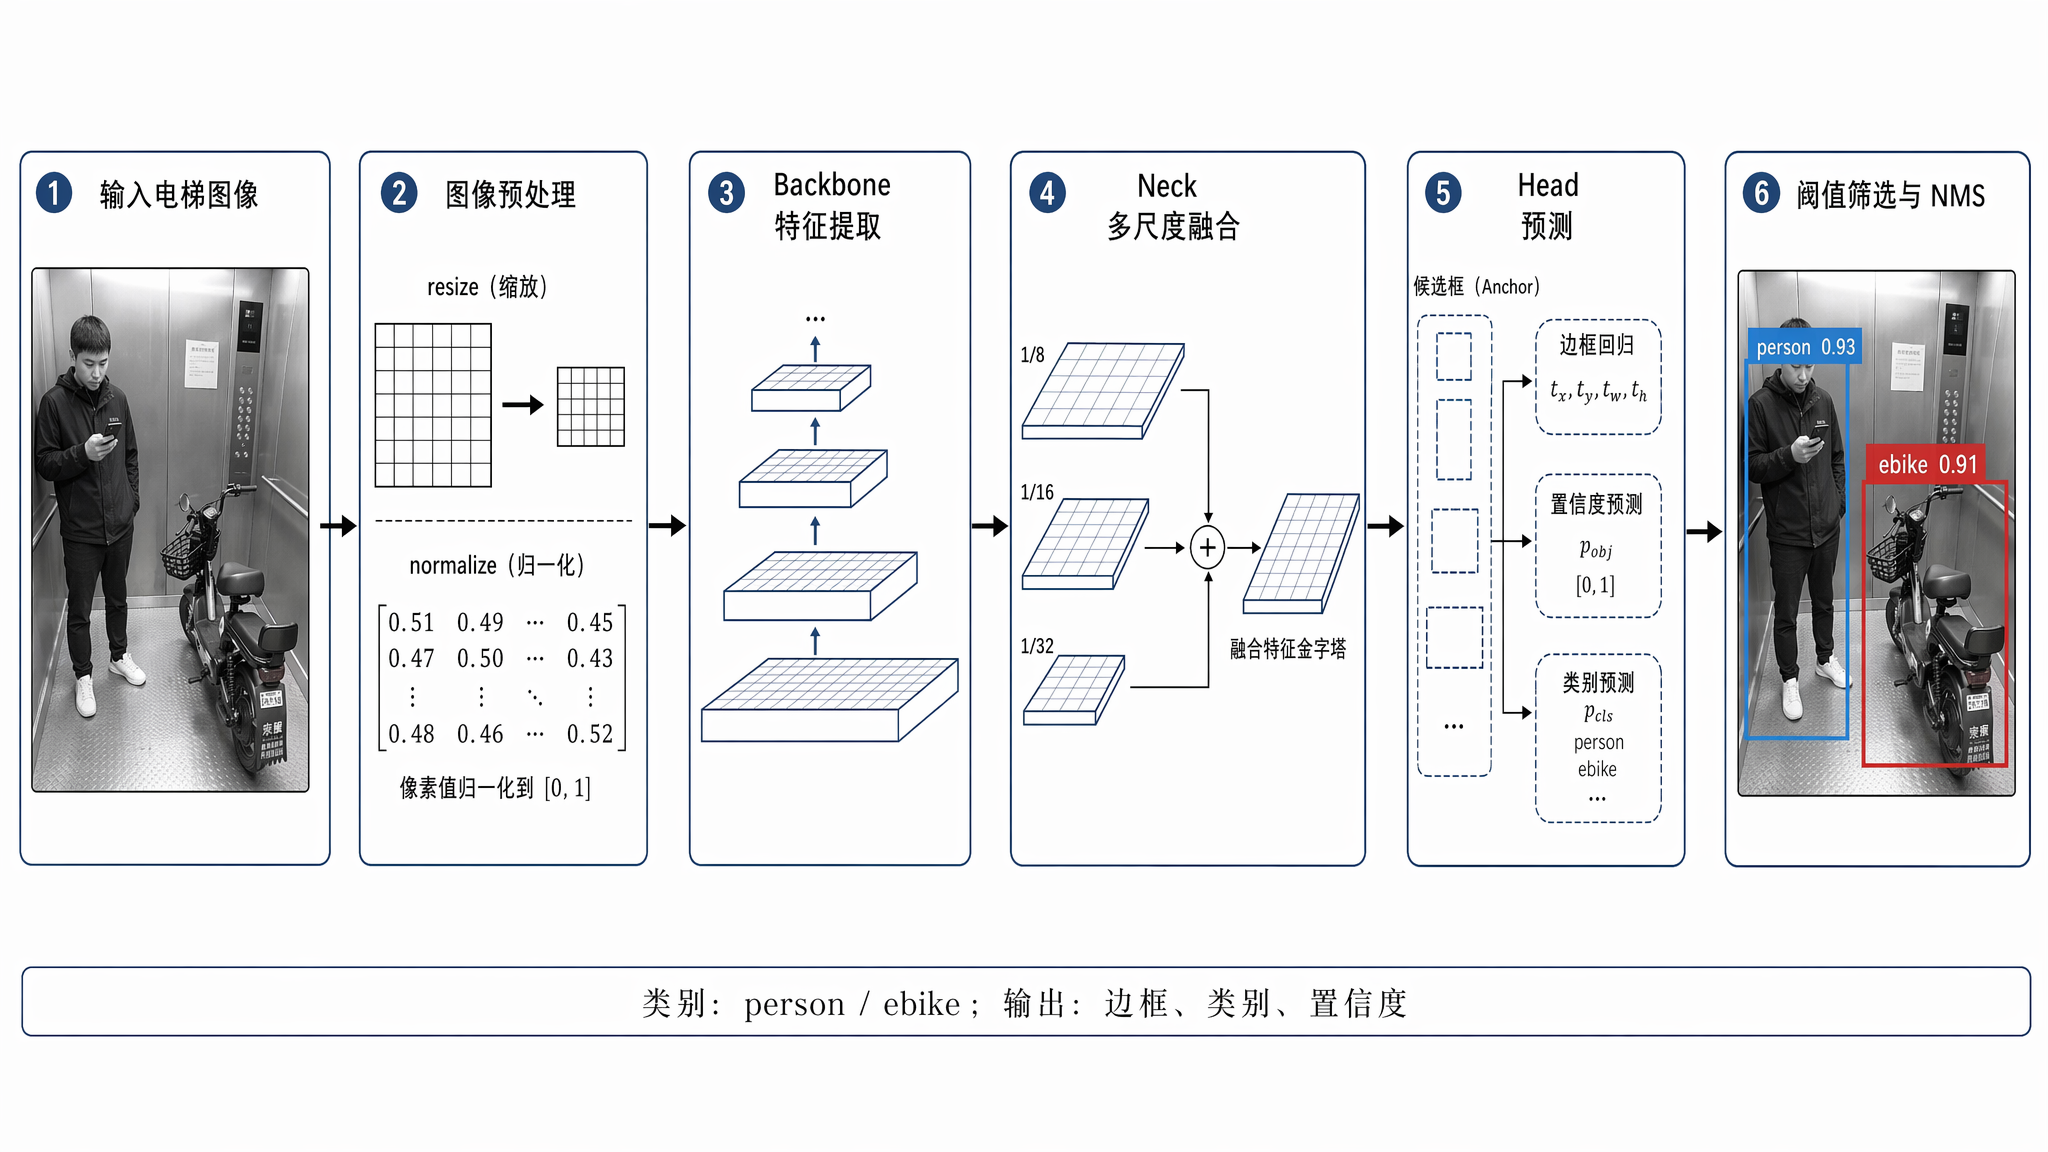
\includegraphics[width=0.92\textwidth]{image/fig2-yolo-pipeline.png}
    \caption{YOLO 双目标检测流程}
    \label{fig:yolo_pipeline}
\end{figure}

本文选择 YOLOv8n，主要是出于工程链路和设备约束的共同考虑。YOLOv8 的训练、导出和推理生态相对成熟，YOLOv8n 的参数量和计算量较小，更适合 HongOU PI 这类边缘开发板。其 anchor-free 检测头和解耦结构也便于检查导出模型的输入输出。虽然 YOLOv9、YOLOv10 等新版本在部分基准上有提升，但本文的双目标任务更看重可部署、可复查和板端适配成本。模型只输出 \textit{person} 与 \textit{ebike} 两类分数；导出后，张量维度、坐标顺序和类别顺序仍必须和板端程序一致。若应用层沿用通用类别数或旧输出格式，即使权重本身没有问题，检测框也可能出现类别错位或坐标失真。

近年来，DETR 等端到端检测框架将目标检测建模为集合预测问题，减少了手工设计候选框和部分后处理步骤\cite{carion2020detr}。这类方法展示了目标检测结构的另一条发展路线，但在本文的边缘开发板场景中，模型部署成熟度、算子支持和实时处理成本同样重要。相比之下，YOLO 系列在工程链路中具有更成熟的导出、编译和板端适配经验，更适合作为本文可复查的边缘安全视觉实现基础。

YOLOv8 的主干、特征融合和检测头边界比较清楚，这有利于检查导出模型的输入输出。但结构清楚不代表部署过程会自动正确。训练框架中的预测结果通常已经完成坐标还原、类别筛选和 NMS；导出到板端后，程序拿到的可能只是未经封装的张量。应用层需要明确张量维度、类别数、分数含义和坐标尺度，否则训练阶段的指标无法和板端检测框放在同一口径下比较。

边框质量也需要统一口径。传统 IoU 衡量预测框与真实框的重叠程度，GIoU 将无重叠情况下的几何关系纳入计算\cite{rezatofighi2019giou}，DIoU 进一步考虑中心点距离\cite{zheng2020diou}。这些指标主要服务训练或离线评测，但它们提醒了一个板端问题：如果坐标解码、缩放或裁剪方式前后不一致，类别分数正常也不能保证 IoU 正常。第三章把边框解释放入接口契约，正是为了避免这类口径错位。

轻量化模型选择需要在精度和设备约束之间取舍。MobileNet、EfficientNet、EfficientDet 等研究讨论了特征提取效率、模型缩放和检测性能之间的关系\cite{howard2019mobilenetv3,tan2019efficientnet,tan2020efficientdet}。电梯场景类别数少，但这并不意味着模型表达能力可以降低要求；遮挡和局部可见目标仍然需要多尺度特征支持。另一方面，边缘开发板的算力和算子支持又限制了模型复杂度。本文采用轻量 YOLO 模型，正是出于检测能力和可部署性的折中。

轻量骨干网络研究为这一选择提供了背景。Inception 结构通过多分支卷积提升表达效率\cite{szegedy2015inception}，ResNet 用残差连接缓解深层网络训练退化\cite{he2016resnet}；MobileNet 系列通过深度可分离卷积和倒残差结构显著降低计算量\cite{howard2017mobilenets}\cite{sandler2018mobilenetv2}，SqueezeNet 以极小参数量实现接近 AlexNet 的精度\cite{iandola2016squeezenet}，ShuffleNet V2 总结了移动端网络设计的实际准则\cite{ma2018shufflenetv2}。MnasNet 和 MobileNetV3 进一步把硬件延迟纳入搜索目标\cite{tan2018mnasnet}\cite{howard2019mobilenetv3}，Once-for-All 则尝试通过一次训练适配多种部署约束\cite{cai2019onceforall}。这些研究共同说明，边缘检测不能只看理论 FLOPs，还需要考虑算子、内存访问和目标硬件的真实执行特性。

在本文任务中，YOLO 的错误往往能在轿厢结构中找到原因。门口的垂直边缘可能干扰边框判断，镜面反光会带来重复候选框，电动车只露出车把或车轮时，分数通常更接近阈值边界。模型结构、数据分布和后处理参数共同决定最终输出。后续实验保留分类别召回率和阈值扫描，目的就是把这些现象落到可以比较的指标上。

\section{边缘部署技术基础}

\subsection{Hi3516DV500 板端 AI 部署基础}

边缘智能强调在靠近数据源的位置完成推理，以降低带宽、隐私和响应时延压力\cite{shi2016edge}。本文使用的 HongOU PI（Hi3516DV500）并非仅作为通用开发板出现，而是作为面向电梯安全视觉的国产边缘 AI 实验平台。该平台搭载华为海思 Hi3516DV500 视觉 SoC，集成双核 ARM Cortex-A55 CPU、专用 NPU、图像处理与媒体输入输出能力，产品规格中给出的典型配置包括 2 GB DDR4、8 GB eMMC 和 2 TOPS INT8 NN 算力。与桌面 GPU 或服务器推理不同，Hi3516DV500 板端部署要求模型先从训练框架导出为中间表示，再通过 CANN/ATC 等工具编译为设备可执行的 OM 离线模型，并在板端应用中通过 SVP\_NPU 相关运行接口完成推理与输出解释。

因此，HongOU PI（Hi3516DV500）在本文中的意义不只是提供运行环境，而是把国产边缘视觉 SoC 的工具链约束纳入研究对象。其部署形态与昇腾生态中常见的“离线模型编译 + 板端运行时调用”工程范式相近，并体现了海思边缘 AI 平台在模型格式、算子支持、内存布局、交叉编译、后处理和运行时接口上的约束。本文选择该平台，是为了在真实板端链路中检验 YOLO 双目标检测模型从训练权重到 OM 模型再到应用输出的语义一致性。图 \ref{fig:ascend_deploy_pipeline} 展示了本文关注的部署链路。

\begin{figure}[htbp]
    \centering
    
\includegraphics[width=\textwidth]{image/fig3-ascend-deploy.png}
    \caption{HongOU PI（Hi3516DV500）开发板上的 YOLO 部署链路}
    \label{fig:ascend_deploy_pipeline}
\end{figure}

这条链路从训练阶段的 YOLO 权重出发，经过 ONNX 导出、ATC 编译与优化，形成 OM 离线模型，再交给板端 NPU 推理。应用层还要继续完成输出解码、阈值筛选和 NMS。链路中的每一步都有可能改写最终结果：预处理差异会改变输入分布，张量读取顺序错误会改变类别语义，后处理阈值不同则会改变检测框数量。

在 Hi3516DV500 板端部署链路中，AIPP、输入尺寸、算子支持和内存布局都会影响模型执行。AIPP 若承担颜色空间转换或归一化操作，则训练阶段预处理必须与板端配置对应；若预处理在应用层完成，则应用层需要保证输入张量与模型期望一致。OM 模型编译完成后，其输入输出名称、形状和数据类型也需要被记录，否则后续调试很难判断错误来自模型本身还是应用层解释。对电梯安全视觉而言，这些约束会直接影响类别顺序、边框解码、候选框筛选和报警稳定性，本文因而把板端工具链和运行时接口作为部署一致性评价的一部分。

深度学习系统研究也表明，模型执行效率不仅由网络本身决定，还由编译器、运行时和硬件体系共同决定。TPU 的系统分析展示了专用加速器在数据中心推理和训练中的性能收益\cite{jouppi2017tpu}，TVM 则代表了通过端到端编译优化把模型映射到不同硬件后端的研究方向\cite{chen2018tvm}。边缘场景与数据中心不同，设备功耗、内存和算子支持更受限制，本文重点关注模型在 Hi3516DV500 板端完整执行后的输出解释和运行口径，而不是把通用加速器吞吐作为主要评价指标。

模型压缩和量化是边缘部署中的常见方法。整数推理友好量化、剪枝和知识蒸馏分别从数值表示、结构冗余和知识迁移角度降低模型部署成本\cite{jacob2018quantization,han2016deep,hinton2015distilling}。混合精度量化研究进一步表明，不同网络层对量化误差的敏感性并不相同，量化策略会影响最终精度和部署效率\cite{dong2019hawq}。不过，本文并不把模型压缩作为主要创新，而是关注场景化训练后的 YOLOv8n 模型在既定边缘平台上的兼容迁移与行为一致性。

量化研究进一步提示，端侧部署中的数值变化需要通过实测而不是假设处理。Krishnamoorthi 总结了卷积网络推理量化中的校准、缩放和整数计算问题\cite{krishnamoorthi2018quantizing}，Gholami 等对高效神经网络推理量化方法进行了系统综述\cite{gholami2021quantization}，AQD 则直接面向量化目标检测的精度问题\cite{chen2021aqd}。这些工作说明，检测模型量化后可能在分类分数、边框回归和候选框排序上产生差异。本文虽然不把量化算法作为贡献，但在实验中区分完整板端验证、阈值后验重算和分段计时，正是为了避免把部署后的数值行为简单等同于训练阶段模型。

\subsection{后处理、NMS 与部署参数敏感性}

目标检测的最终输出并不完全由神经网络前向结果决定。置信度阈值决定候选框是否进入后续统计，NMS 决定重叠框的保留关系，类别特定的清理规则则可能改变某一类目标的误报和漏报。Soft-NMS 表明，即使只改变传统 NMS 的抑制方式，也可能改善检测结果\cite{bodla2017softnms}。对于本文的电梯场景，NMS 的影响更具体：人和电动车经常在狭窄空间中重叠，电动车局部结构又可能生成多个相邻候选框，过强或过弱的抑制都可能改变最终安全输出。

本文不把阈值、NMS 和后处理策略简单看作“调参”。训练脚本与板端应用若采用不同置信度阈值，precision、recall 和预测框数量都会变化；NMS 阈值一改，拥挤重叠区域的候选框保留关系也会随之改变。应用层若增加类别特定清理规则，某些看似模型能力不足的问题，实际可能来自候选框处理。第五章中的阈值扫描、NMS 实验和后处理消融，正是为了把这几类影响拆开。

把后处理作为部署模块单独讨论，可以分清模型前向结果和应用层规则的边界。本文先报告端到端板端基准，再用参数敏感性和消融实验解释关键设计选择。这样写，是为了说明模型权重、阈值、NMS 与电动车清理规则如何共同决定最终输出。

边缘部署还要区分“能够运行”和“适合应用”。前者只说明模型可以编译、加载和推理；后者还要求输出含义清楚、失败样本有迹可循，后处理规则也要符合安全任务。本文在结果章同时报告成功样本数、batch 验证链路耗时、分段计时和阈值扫描，把板端可运行性拆成检测输出、验证链路和耗时口径几个可检查部分。

\section{相邻视觉任务与本文重点}

电梯轿厢内的安全视觉任务可以按观察尺度分成不同方向。轿厢拥挤程度通常要落到人数统计上，已有研究把边缘轻量检测器用于电梯人数统计系统\cite{lin2023elevatorcounting}。当问题转向目标在多帧中的持续状态时，DeepSORT、ByteTrack 等跟踪方法才成为主要工具\cite{wojke2017deepsort,zhang2022bytetrack}。姿态估计和视频识别还能给出人体关键点或动作模式\cite{cao2017openpose,feichtenhofer2019slowfast}，不过这些任务会引入视频级标注、时序模型和行为定义。本文的实验范围因此收束在 \textit{person} 与 \textit{ebike} 的板端检测，而不是把跟踪和动作识别一并纳入主线。

连续视频在本文中承担的是补充检查作用，用来观察单帧指标不容易暴露的框保持、闪烁和耗时波动。跟踪方法本身已有较成熟的处理路径：SORT 用卡尔曼滤波预测目标状态，再通过匈牙利匹配连接相邻帧检测框\cite{bewley2016sort}；DeepSORT 在此基础上加入外观特征，以改善跨帧身份关联\cite{wojke2017deepsort}；ByteTrack 则把部分低分检测框保留下来参与关联，减少轨迹断裂\cite{zhang2022bytetrack}。这些设计关注的是检测结果在时间轴上的延续关系，与本文的单帧双目标检测评价并不属于同一层级。因此，代表性视频片段只用于补充观察连续输出保持、闪烁和分段耗时，为板端部署一致性提供场景证据。

后续章节仍围绕图像级双目标检测和板端迁移展开；跟踪或动作识别可以作为后续扩展，但不放入本文的主要实验链路。

\subsection{部署一致性问题}

本文所说的部署一致性，指同一检测模型经过格式转换和设备迁移后，输入、输出和后处理仍处在可比较口径下。普通离线实验往往关注最终 mAP；安全视觉系统则不同，类别错位、边框漂移、阈值变化或运行时异常都可能改变预警结果。因此，这一问题不能只写成实验环境说明，而要进入方法设计。

在本文中，需要核对的内容包括类别、边框、阈值和运行记录。类别顺序要在训练、ONNX 导出、OM 编译和板端应用之间保持一致；坐标归一化、缩放和裁剪方式要能支撑同一套 IoU 判断；置信度阈值与 NMS 参数在不同阶段应表达相同含义；设备端还要记录成功样本数、失败样本数、batch 端到端耗时和分段计时。少了其中任何一项，板端指标都可能被误读。

这些检查项之间存在前后依赖。类别顺序错误时，precision 和 recall 的语义会失效；坐标还原错误时，模型可能被误判为定位能力不足；阈值口径不一致时，安全输出会受偶然参数影响；运行记录不足时，一次实验也难以代表真实设备行为。第二章先把这些问题说清楚，第三章再给出接口契约，实验章据此解释结果。

已有部署研究指出，深度模型从训练框架迁移到生产环境时，格式转换、算子支持和运行时差异会带来额外风险\cite{stacker2021deployment,chen2021aqd}。电梯场景会把这种风险放大：反光和门口结构使候选框分数更容易贴近阈值，局部可见电动车会让边框更敏感，拥挤重叠也会影响 NMS。后续方法章围绕接口契约和分阶段验证展开，就是为了把这些风险落到可检查的技术项上。

\section{相关工作小结}

本章的技术背景指向一个明确缺口：YOLO 系列适合作为电梯双目标检测基础，边缘 AI 平台也具备本地预警的硬件条件；但既有工作常把检测精度和边缘部署分开讨论，较少把训练权重、ONNX 中间表示、OM 离线模型和板端后处理放在同一条证据链里。本文以行人与电动车检测为任务载体，面向 HongOU PI（Hi3516DV500）开发板整理兼容迁移方法，并在后续章节用板端实测结果检验这条链路。
